\documentclass[a4paper]{article}

\usepackage{natbib}
\bibliographystyle{authordate1}

\usepackage{INTERSPEECH2022}
\usepackage{amsmath,graphicx}
\usepackage{mathtools, nccmath}
\usepackage{graphicx}               % Necessary to use \scalebox
\usepackage{amsmath,amssymb}
\usepackage{color,soul}
\usepackage{caption}
\usepackage{url}
\usepackage{adjustbox,lipsum}
% Example definitions.
% --------------------
\def\x{{\mathbf x}}
\def\L{{\cal L}}

\makeatletter
\setlength{\@fptop}{0pt}
\makeatother

%\setcitestyle{authoryear, citesep={&}} %Citation-related commands
%\usepackage{apacite}

\usepackage{hyperref}
\hypersetup{
  colorlinks   = true, %Colours links instead of ugly boxes
  %urlcolor     = red, %Colour for external hyperlinks
  linkcolor    = blue, %Colour of internal links
  citecolor   = blue %Colour of citations, could be ``red''
}

\title{Automatic Chord Detection}
\name{Daniel Gilkarov$^1$}

\address{
  $^1$School of Computer Science, Ariel University, Israel}
\email{dgilkarov33@gmail.com}


\begin{document}
\maketitle

%\twocolumn[
%  \begin{@twocolumnfalse}
%    \maketitle
    \begin{abstract}
      Automatic Chord Recognition (ACR) is a field with various uses among the music industry, with rapid growth in digital networks centered around music rises a great need for music analysis tools. One way of analysing music is through the chords that make it up, most western pop songs are composed with 3-4 chords. The necessity of ACR is assured through the inclusion of ACR as MIREX tasks since 2019. This paper presents a CNN based system  built upon previous work with robustness of the model to different musical instruments achieved using various data augmentation techniques. The model's abillity are further demonstrated using an Out of Distribution (OOD) dataset consisting of audio that's quite different from the training data.
   \end{abstract}
%  \end{@twocolumnfalse}
 %       ]
\section{Introduction}
Music is one of the most prominent forms of art, dating back even before spoken language existed \cite{music_before_language}. Throughout the times, humans have used music for expressing themselves, having music evolve together with us as a species \cite{music_human_evolution}, from the early stages of tribal music all the way to modern electronic music which now dominates the billboards and our ears.

People find great interest in learning to play musical instruments, with a very broad range of instruments and countless niches - string instruments played by plucking strings - for example of course the guitar which is one of the most popular instruments, with 712 million people worldwide having touched a guitar - \citeauthor{guitar_players_amount} - this is about 8.6\% of the world population \citep{world_population}

Moving on there are also percussion instruments such as drums - which are also an integral part of a lot of types of composed music, and historically, it was observed that lots of ancient civilizations used these kinds of instruments one way or another \cite{percussion_ancient}.
Another popular type of instruments are wind instruments, played by blowing air into the instrument, and usually manipulating the notes that ring out by blocking out certain pathways the air escapes through \citep{wind_instruments}, this is just the tip of the iceberg.

It can be seen that music through this, is something so versatile, so universal, great musicians around the world were granted great ranks of honor as appreciation of their talent \citep{music_honor_wiki}, for example, Mozart, a musician that's as well known as Einstein, long after his death.

In more modern times, with the internet - people use the it among all its other uses for learning to play instruments, sharing their passion for music with others, sharing their music that they created with others \cite{internet_music}.
With a large amount of people that rely on the computer for learning their instrument, arises a need for an effective way to teach music, store music, play it using the computer.

In order to allow computers to store data about music, an intermediary called Musical Instrument Digital Interface (MIDI) was born \citep{midi_wiki}, a digital interface and "language" for representing structured music inside the computers memory.

Seeing as music is so popular, many companies and organizations were founded centered around it, with the music industry valued around \$26.2 billion \cite{music_industry_worth}
Radio stations, Music studios, Companies that develop applications that deal with music, such as instrument teaching apps, song recognizing apps, audio streaming platforms and more.

These are all organizations that have a need for a systematic way of characterizing music pieces \citep{music_industry_wiki}, for example, radio stations may want to choose which songs are most likely to be liked by their audience, music teaching apps usually work nowadays by listening to someone play and giving them feedback, and so these kinds of apps need a way to tell someone if they're playing correctly or not and if not describe what's the problem.
One way of analysing a music piece is through the chords that make it up using \textbf{Chord Recognition}.

Most modern western music is composed using chords and melodies played with chords \citep{musictheory_wiki}, knowing the chords of a song can help us in other tasks of music analysis, such as finding the key of a song, which is the group of notes, or scale that forms the basis of a music piece. Knowing the key can help us group songs together, help us have a general understanding of how they'll sound, since the key dictates the notes that are used in the song, some songs change keys mid-song and this kind of composition style is very popular with jazz music, with the feel of the song mutating and evolving as the song goes on.

A chord is a set of three or more notes that are played at the same time. Chords are built upon a certain note, known as the root note, which defines the chord, for example a D-minor chord has the note D as its root \citep{chord_wiki}. There are 2 major types of chords, major and minor, with major chords usually sounding happy and uplifting, minor chords which sound sad and melancholic \citep{musictheory_wiki}. The difference between them lies in the interval between the notes that make up the chord.
An octave is the interval between one note and another with double its frequency.
Most musical scales are written so that they begin and end on notes that are an octave apart. For example, the C major scale is typically written C D E F G A B C. the initial and final C's being an octave apart.
Tuning is the process of adjusting the pitch of one or many tones from musical instruments to establish typical intervals between these tones. 
The most common tuning system since the 18th century has been 12-tone equal temperament

Chord Recognition deals with recognizing chords played inside audio tracks, and providing information about which chords were played and when, a task which is sometimes given to people to do, stated as one of the Music Information Retrieval Evaluation eXchange (MIREX) tasks \cite{mirex}.
ACR on the other hand, tries to automate this process with the use of computers.

This technique faces several challenges: songs usually have multiple instruments playing slightly different melodies, audio files are processed more than before, some chords and notes bear great similarity and machines some times struggle to discern them, to recognize the chord there's a need for identifying the root note and sometimes the notes are inseparable.

ACR has applications in various situations:
It's used in song analysis, where the chords are extracted to help characterize it, because they sometimes play a big role in creating the whole experience of the song, it can be used to measure similarity between songs. Using it this way can assist in creating for example a song recommendation system, to recommend songs to users of an app that serves music based on their melody, portrayed through the chords.
These kinds of techniques are also useful on their own in systems that aim to teach users to play an instrument interactively, giving feedback on whether the right chord was played on various levels of verbosity. Audio search engines can use ACR to identify songs based on the chords that are recorded.

Of course this method is not without its downsides, many times a song isn't exclusively made up of chords, often there are melodies comprised of individual notes. This means that this method isn't enough on its own to paint a full picture, rather it is one tool in the toolbox of music analysis. Moreover, ACR usually relies on some kind of structure, both in that chords themselves are well-defined repeating entities, and also that the song, or music piece is composed with common sense (this can be argued to be inevitable), for example that there aren't 5 different chords overlapping at one point in the track, this makes it more difficult to deal with for instance, orchestral music, where not only it's impossible to say that from 03:05 to 03:10 a BMaj chord was played, maybe it's more like 03:05-03:07 - Bmaj, 03:02-03:09 - Amin, and so on.

ACR systems follow two distinct steps from start (Raw Audio input) to finish (Segmented timeline into chords labels and duration) most of the time: feature extraction and pattern matching. 
For feature extraction the audio signal is cut into short frames and each frame is transformed into an harmonic feature vector.
Afterwards in pattern matching each frame is fit a chord label by measuring the similarity between its harmonic features and predefined chord models.
Many systems also go further to introduce additional filtering steps aimed at dealing with errors that happen in the first and second steps, there's pre-filtering that takes place before the second step and post-filtering that happens after the second step.
ACR solutions proposed in academic literature largely follow this structure, varying between different feature extraction techniques, different pattern matching techniques, with/without pre/post-filtering with varying techniques and different chord models ranging from the most basic model and some with great complexity.

Ever since ACR solutions started appearing, in terms of the feature extraction phase - chroma features are the most used features for it to this day.
A chroma feature vector, also called pitch class profile (PCP), represents the energy distribution of a signal’s frequency content across the 12 pitch classes of the equal-tempered scale.
A temporal sequence of these chroma vectors is often called a chromagram.
Another closely related option for representing audio with respect to time like PCP is a spectrogram, a spectrogram is a visual representation of the spectrum of frequencies of the audio signal as it varies with time. In practice these spectrograms are 2D representations of audio and are often used together with CNNs (Convolutional Neural Network) for ACR \cite{cnnacrspectro}, these CNNs have been found to deal with image data very effectively through the action of convolution, using kernels or filters that slide along input features and provide feature maps.
As a chord is made up of a set of notes and it's assumed that the chord label can be determined by the occurrence of notes no matter in what octave, chroma features are still used to this day, and feature extraction is refined and improved through variation on the commonly-used chroma vectors.
In terms of models used for the chord classification, there's an ever-growing use of deep-learning models such as CNNs , DNNs (Deep Neural Network).

For pre-filtering, most times the chromagrams are augmented before the chord labelling process, usually aiming to blur out noisy frames by smoothing the features across neighboring frames, typically done using moving average filter or moving median filter.

With regards to the pattern matching and post-filtering phase, Some use discriminative ML (machine learning) techniques such as CRF (Conditional Random Field) \cite{crf1}, in recent years with the advancement in deep-learning there's more and more use of CRF along with some kind of deep-learning model for feature extraction: 
\cite{crf2} used a CNN for feature extraction along with CRF and BLSTM (Bidirectional Long Short-Term Memory), \cite{crf3} experimented with a DNN for chord labelling and compared performance of various RNNs (Recurrent Neural Network) (LSTM, Bi-LSTM, GRU (Gated Recurrent Unit)) for post-filtering.
Some use SVMs (Scale Vector Machine), in \cite{svmVHMM} SVM was compared against HMM (Hidden Markov Model) for post-filtering.
there is repeated use of HMMs for post-filtering 
these describe the dynamic behavior of features in terms of transitions between chords. The transitions are dictated by a group of probabilities called transition probabilities that describe the likelihoods of transiting from a chord to another. An algorithm called Viterbi finds the most likely chord sequence by evaluating the joint probability of the output from the pattern matching stage and all possible chord sequences based on a given transition matrix. This in turn reduces the number of false chord predictions by restricting unlikely chord transitions.

\subsection{Our Contribution}
This article offers a robust approach for ACR capable of recognizing chords played in various different instruments in contrast to the baseline model which is only trained on guitar recordings and shown to very ineffective with instruments that aren't guitar. The proposed approach is also shown to be able to train very quickly in comparison to the baseline and at the same time have performance on par with the baseline in the data it is specially trained for (guitar recordings).

\subsection{Paper Structure}
The remainder of this paper is structured as follows: Section \ref{sec:related_work} surveys related work mainly regarding common ACR approaches in general, and Deep Learning (DL) solutions in particular; Section \ref{sec:dataset} discusses datasets used in this paper and the pre-processing procedure; Section \ref{sec:data_aug} presents the different data augmentation methods that were utilized in this work; Section \ref{sec:framework} presents the approach employed in this paper; Section \ref{sec:experiments} presents a fine-grained experimental evaluation process, that consists of an evaluation of our augmentation-based ACR approach, and the results of the comparison between our approach and a CNN baseline version; Finally, Section \ref{sec:conclusion} concludes the paper and offer some directions for future work.
For ease of reading, Table \ref{tab:list_of_abbreviations} provides a list of abbreviations that are commonly used in this paper.

\begin{table}[th]
\caption{List of abbreviations}
\label{tab:list_of_abbreviations}
\centering
\begin{adjustbox}{width=\columnwidth}
    
      
      \begin{tabular}{ |c|c|c|}
      \hline
        \multicolumn{1}{|c|}{\textbf{Abbreviation}} & 
        \multicolumn{1}{|c|}{\textbf{\# Meaning}}\\\hline
        ACR & \quad Automatic Chord Recognition  \\\hline
        BLSTM & \quad Bidirectional Long Short-Term Memory \\\hline
        CE & \quad Cross Entropy  \\\hline
        CNN & \quad Convolutional Neural Network  \\\hline
        CRF & \quad Conditional Random Field  \\\hline
        DL & \quad Deep Learning  \\\hline
        DNN & \quad Deep Neural Network  \\\hline
        GRU & \quad Gated Recurrent Unit  \\\hline
        HMM & \quad Hidden Markov Model  \\\hline
        MIDI  & \quad Musical Instrument Digital Interface \\\hline
        MIREX & \quad Music Information Retrieval Evaluation eXchange \\\hline
        ML & \quad Machine Learning  \\\hline
        PCP & \quad Pitch Class Profile  \\\hline
        RMS & \quad Root Mean Square  \\\hline
        RNN & \quad Recurrent Neural Network  \\\hline
        SNR & \quad Signal to Noise Ratio  \\\hline
        STFT & \quad Short-time Fourier transform  \\\hline
        SVM & \quad Scale Vector Machine  \\\hline
        
      \end{tabular}
    
\end{adjustbox}
\end{table}

\section{Related Work} \label{sec:related_work}
Initially, Chord Recognition was performed by calculating chroma features \citep{1999}, then labeling chords by template matching against models of known chords.
Chroma features, despite being very widely used in this field tend to be noisy, and in the context of specifically looking for chords, sometimes these chroma features contain scattered notes which can't be recognized as chords.
This leads other researchers to incorporate different types of auxiliary features, such as temporal continuity \cite{temp1, temp2}.
Other features used include various musical properties such as beats \cite{temp2, beat1}, key \cite{key1}, bass \cite{bass1}.

In \cite{featcompare} the importance of different features and data manipulation techniques for ACR are systematically investigated, revealing a great importance for using pre and post filtering, where in pre-filtering typically blurring out noisy frames by smoothing the features across neighboring frames before the pattern matching phase. post-filtering is usually applicable in HMM-based chord recognition systems. The above methods are shown to greatly improve accuracy.

The use of DL models is seen to increase in recent years and show promising results in ACR, usually used as part of a pipeline for feature extraction, CNNs are often used \cite{cnn2012, cnn2016} - showing performance not far from the state-of-the-art, with a computational expense that's associated with CNN's, \cite{cnn2021} aims to this tackle this issue by suggesting what they call a "FifthNet", in their words a compact CNN that achieves similar results to other CNN-incorporating systems with much lower computational requirement.

There is recurrent (pun intended) use of RNNs for sequence modelling in text, speech, video domains, mainly through the means of LSTMs and for our purpose, in music transcription, ACR and so on \cite{rnn2013, lstm2017}.
\\
In this article we take a chord recognition system, designed for classifying short recordings of guitar sound to a range of 10 chords \cite{baseline}. This chord recognition system has good results classifying guitar chords from a dataset curated by MONTEFIORE RESEARCH GROUP of university of Liège - recall: 91\%, precision: 94\%, f1-score: 92\%
We aim to make this system more robust to different sound other than guitar, for example: the baseline model performed poorly on piano recordings from the same dataset - recall: 21\%, precision: 22\%, f1-score: 21\%

\section{Datasets} \label{sec:dataset}
The datasets used in this paper are summarized in Table \ref{tab:list_of_datasets}, it provides the total dataset duration and total number of chord segments.
\\
Table \ref{tab:class_amounts} provides amounts of samples of each class for each dataset
\\

\noindent In this article, 2 datasets were used, one in training and one for testing:

1. \textbf{Osmalsky}: a dataset created by MONTEFIORE RESEARCH GROUP of university of Liège \cite{dataset, dataset_ood, baseline} is used for training the model. The dataset is a free publicly available collection of isolated recorded samples of chords played on guitar, accordion, violin and piano
This dataset is comprised of 2 second long WAV recordings sampled at 44100 Hz.

Originally the creators of the datasets meant this dataset to be a guitar chords dataset, with the rest of the recordings of the other instruments meant to be used as a test set to prove their ML algorithm's ability to generalize to other instruments, in this article however we will make use of these samples to train our DL model - to counter the fact that the dataset is greatly unbalanced between the guitar recordings and the others, we utilize data augmentation.
The chord recordings are distributed equally between 10 different chord classes:
\begin{center}
    A, Am, Bm, C, D, Dm, E, Em, F, G
\end{center}

There are 200 chord recordings of each class for the guitar recordings and 10 recordings of each class for the other instruments.
This dataset (like a lot of others with the same niche) was created with the aim of matching to some degree the sound of western pop music, in their article they claim this was also the motive behind choosing these chords specifically and the guitar as the main recording instrument.

The guitar recordings were recorded using 3 different acoustic guitar(s) and a nylon string guitar - half in an an-echoic chamber and half in a noisy environment in order to simulate real life scenarios for artists recording (Studio and Live performances), moreover the recordings were played in several different playing styles - (arpeggio, staccato, legato, etc.). These varieties in recordings are meant to offer a more wide range of sound to help models learning this data become more robust.\\
\begin{table*}
\centering
\begin{adjustbox}{width=\linewidth}    
\begin{tabular}{c c c c c} % creating 10 columns  
\hline   
 Dataset & Duration (h) & \#Chord Samples  & Sample Duration & Sampling Rate\\
\hline\hline
% Entering 1st row  
Osmalsky & 80 & 2400 & 2 seconds & 44.1 KHz\\
IDMT-SMT-Chords & 5.3  & 160  & 2 seconds & 44.1 KHz\\
\hline
% [1ex] adds vertical space  
%\hline % inserts single-line  
\end{tabular}  
    
\end{adjustbox}
\caption{Overview of the chord recognition datasets with
the total duration in
hours, the number of chord samples, sample duration per dataset and sampling rate.
In order to enlarge the training dataset (Osmalsky), we use time-stretching (2 variants) and additive gaussian noise (3 variants) as data augmentation technique. Hence, each original file
results in 5 augmented files including the original recording. 
}
\label{tab:list_of_datasets}
\end{table*}
\begin{table}
\centering
\begin{adjustbox}{width=\columnwidth}
    
      
\begin{tabular}{c c c c c}
\hline   
 Dataset & Guitar & Piano & Accordion & Violin \\
\hline\hline
% Entering 1st row  
Osmalsky & 200 & 60 & 60 & 60\\
IDMT-SMT-Chords & 6 & 10 & 0 & 0 \\
\hline
% [1ex] adds vertical space  
%\hline % inserts single-line  
\end{tabular}  
    
\end{adjustbox}
\caption{Overview of amounts of chord samples per class for each dataset
}
\label{tab:class_amounts}
\end{table}

2. \textbf{IDMT-SMT-Chords }:
Synthetic dataset \cite{dataset_ood} created using Ableton Live and Garage Band, the dataset consists of 2 second long samples of MIDI chords. The chords are played in the following chord voicings which are commonly used on keyboard instruments and guitars:

\noindent Ableton Live:
\begin{itemize}
    \item Campfire Guitar
    \item Guitar Open
    \item Nylon Concerto Guitar

    \item Celestial Pad
    \item Grand Piano Reverb
    \item Grand Piano
    \item Piano to Pad
    \item Sadness Pad
    \item Sweetness Pad
\end{itemize}

\noindent Garage Band:
\begin{itemize}
    \item Acoustic Guitar
    \item Hard Rock Guitar
    \item Classic clean Guitar

    \item Boesendorfer Grand Piano
    \item Deluxe Modern Piano
    \item Jazz Organ
    \item Steinway Grand Piano
\end{itemize}

The dataset was created to remedy the scarcity of datasets with 7th chords but this article doesn't aim to classify 7th chords and therefore only the chords which are relevant here were extracted from the recordings.
Out of the \textbf{7398} audio segments we end up using \textbf{160}, as mentioned in table \ref{tab:class_amounts} we have 6 audio samples of every class generated using 6 different \emph{guitar} sounds available in the programs mentioned and 10 audio samples of every class generated using 10 different \emph{piano/keyboard} sounds, one sample per each different chord voice.

While the samples in the training set are very organic (being played by a human on a real instrument and recorded in simulated scenarios) and vary mostly through the way the chords are played (arrpegiated, strummed, etc.), its is appearent that in contrast the test set is created artificially (which standardizes the sound produced) contains samples with great in-dataset variety due to the fact that for every chord class we have one sample of each instrument preset in the MIDI software with some presets producing sounds resembling synthesizers. This means the test dataset is very different from the training data - this is good since the testset being very different from the training set provides a better test for robustness of a ML model.


\subsection{Pre Processing} \label{ssec:preprocessing}
The preprocessing phase starts off by taking the raw WAV files, constructing a dataframe where each row represents one sample in the dataset. For each sample the label is also included, one of the classes detailed in section \ref{sec:dataset}.
\subsubsection{Mel Spectrogram} \label{sssec:mel-spectrogram}
The main feature that's fed into the CNN model propsed in this article is a mel-spectrogram.
Mel-spectrograms are spectrograms where the frequencies are converted to the mel scale.
Humans hear frequencies logarithmically rather than linearly. And so,
a 100Hz difference in the Mel Scale corresponds to what
a human would typically perceive in the actual world. So the mel-spectrogram deals with the issue of the spectrogram not reflecting change in frequency as a human would, the mel-scale converts a tone’s perceived frequency to its actual frequency.
Mel spectrograms hold sound information which the human ear could perceive. The Mel scale and Hertz(Hz) are
related by the given formula:
\[ m = 2595\log_{10}(1 + \frac{f}{700}) \]
For every sample a mel-spectrogram is calculated (window length - 2048) using the librosa python library which calculates a Short-time Fourier transform (STFT) .
The largest shape of these spectrograms present in the whole dataset is found and the spectrograms are zero padded from the right to achieve a uniform shape.
Every mel-spectrogram is scaled using the log function \cite{lognorm} in the following way: \[log(X + \alpha)\] where alpha is an arbitrary small number like $10^{-7}$ or 1 and X is an input mel-spectrogram. This article uses $\alpha = 10^{-7}$.

\subsubsection{Data Normalization}
This article takes advantage of data normalization to allow the model to converge more quickly by reducing the variety of spectrograms frequencies across different instruments. Nomalization makes the data distribute in a more gaussian fashion, therefore making the data more balanced and prevents outliers which makes the data skewed and often hurts the learning process.
The log-mel-spectrograms are normalized so that all the values lie in the $[-1, 1]$ by taking each row of a spectrogram and dividing every value by the maximum value of the row: \[X_{normalized} = \frac{X}{max(X)}\]
% Every spectrogram we calculate is normalized using log-normalization - this has quite a few effects on our framework, in contrast with our baseline model which was trained for 70 epochs, our model reaches a similar performance after 8 epochs. This data normalization also helps prevent the model overfitting our data as is shown later in the experiments section.


\section{Data Augmentation} \label{sec:data_aug}
Data augmentation \cite{augment1, augment2} is a common technique that is used to artificially increase the
size of a dataset by creating modified versions of existing data. In the realm of audio, this can be done by applying
transformations such as pitch shifting, time stretching, or adding noise to the audio clip.
Data augmentation is often
used in machine learning and especially deep learning where most of the time the crucial make-or-break point of a DL model is it's access to good quality diverse data. Data augmentation is used to improve the performance and generalization of models by providing them with additional
training examples. The new augmented data is viable since the augmentations do not interfere with the transcription
of the original audio-recording and usually can be label-perserving which is important for supervised learning systems. The new data can be used to further train the model.
Focusing on a minimal number of high-impacting augmentations which introduce variance that's maybe lacking in the training data is vital to successfully improving the model, when using augmented data - being able to maintain good performance on test data which wasn't augmented is vital since if there's success with augmented data but failure with real data - there isn't real value in such improvements. In this work, two augmentation methods are considered:
\begin{itemize}
\item Gaussian-Noise \cite{augment_noise} (section \ref{ssec:noise})
\item Time-Shift \cite{augment_time1, augment_time2} (section \ref{ssec:time})
\end{itemize}

\subsection{Gaussian Noise} \label{ssec:noise}
Artificially adding Gaussian-Noise augmentation to the training data can improve ¨
the robustness and generalization of an ACR model. The goal of this method is to make the model more resistant
to variations in the input data such as the differences between sounds of different instruments, in addition it helps by simulating real-world scenarios where the data is noisy in contrast with studio-recorded data with perfect conditions.
In order to augment the audio-recording and add noise, first noise is generated based on a certain Signal to Noise Ratio (SNR) value - SNR is given by: 
\begin{equation}
   SNR = 10log(\frac{RMS_{signal}^2}{RMS_{noise}^2})
   \label{eqn:snr}
\end{equation}

\noindent where for a group of n values involving {x1, x2, x3,…. Xn}, the Root Mean Sqaure (RMS) is given by:
\begin{equation}
RMS = \sqrt{\frac{x_1^2 + \dots + x_n^2}{n}}
\label{eqn:rms}
\end{equation}

\noindent when generating noise, given some SNR value, the $RMS_{noise}$ is calculated and random gaussian distributed values are generated with standard deviation equal to it, then adding the original signal and the noise arrays resulting in the original audio with noise added to it with the volume of noise dictated by the SNR value.

\subsection{Time Stretching} \label{ssec:time}
The audio sample is speeded up or slowed down without changing pitch. This prevents the model from overfitting to a certain tempo when regarding music in general and more specifically, chords played on string instruments, by creating audio samples which are faster (by a factor of 1.07) and slower (by a factor of 0.81) the aim is to increase general robustness - the model will have to be able to deal with the audio with varying speeds and therefore be more ready to tackle real-life audio samples with varying speed.
The time stretching is implemented using librosa.effects

% We use data augmentation for 2 reasons:

% 1) Further diversifying the dataset - causing the model to overfit less and get overall better results after training

% 2) Fixing the imbalance in the dataset between the amount of guitar samples and the other instruments (accordion, violin, piano) - for this purpose we apply data augmentation only to the other instruments' samples and not the guitar samples.

% We take the data augmentation techniques suggested in the baseline article and further improve upon them.
% In total we perform 5 data augmentations:

% 1) Time Stretch - we do 2 different augmentations by stretching and compressing the audio, this results in 2 more copies of every recording, one x1.07 faster and one x0.81 slower.

% 2) Gaussian Noise - by adding white noise to recordings we increase the model's ability to cope with noisy recordings whenever the original data is not noisy and recorder in a good studio environment for recording which sometimes doesn't reflect real-life recordings often made in crowded places like live venues, etc. We take each recording and add 3 levels of noise to it - 10db, 20db and 30db of noise.

\section{Framework} \label{sec:framework}
\begin{figure*}[t]
\centering
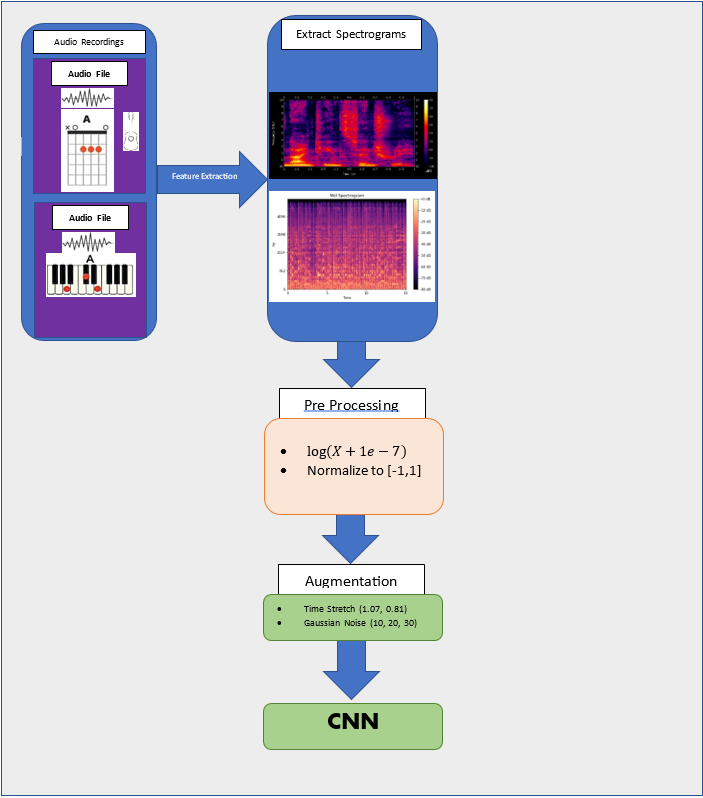
\includegraphics[width=\textwidth]{figure1.png}
\caption{An illustration of the suggested framework in this paper. For any audio recording of musical instruments, the mel-spectrogram is extracted as detailed in section \ref{sssec:mel-spectrogram}. The mel-spectrogram is transformed using the log function as detailed in section \ref{ssec:preprocessing} and then normalized to the range [-1, 1]. The data is then augmented using Time Stretching and Gaussian Noise addition and finally fed into the CNN.}
\label{fig:img1}
\end{figure*}

\begin{figure}[!h]
% \centering
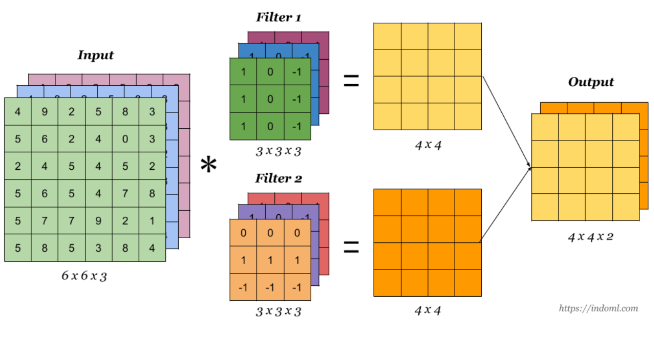
\includegraphics[width=.5\textwidth]{convolution.png}
\caption{Convolution operation - the basic operation used in Convolutional Neural Networks.}
\label{fig:conv}
\end{figure}

The following section describes the method proposed by the article for doing ACR on audio samples containing one chord - labeling them as one of predetermined classes, see section \ref{ssec:classes} for reference.
In section \ref{ssec:system_description} the general structure and data-flow of the models is laid out.
In section \ref{ssec:model_architecture} the models are discussed with greater detail, also presenting the motivation for the proposed actions. 
\subsection{Classification Classes} \label{ssec:classes}
The classification classes for the chords in this system are: 
\begin{center}
    A, Am, Bm, C, D, Dm, E, Em, F, G
\end{center}
\subsection{System description} \label{ssec:system_description}

The main architecture of the model has three main building blocks (See figure \ref{fig:img1} for reference):
\begin{itemize}
    \item \textbf{Pre-Processing} The model receives raw audio file in WAV format as input and it calculates a mel-spectrogram of it, then applying log to every value in it and finally normalizing it to the range [-1, 1]. See section \ref{ssec:preprocessing}.

    \item \textbf{Data augmentation} Every sample (except samples of guitar sound) in the processed dataset is applied Time Stretch and Gaussian Noise data augmentations to get in turn 5 different augmented samples of each sample. See section \ref{sec:data_aug}

    \item \textbf{Chord Classification} The data is input into the CNN where it gets classified as one of the 10 predefined classes defined above.
\end{itemize}

\subsection{Model Architecture} \label{ssec:model_architecture}
The baseline model which this article builds upon \cite{baseline} consists of a CNN.
This article proposes two models and investigates their performance side by side.
The first model is identical in its architecture to the baseline model, the second model is similar with the dropout \cite{dropout} layers taken out.\\
The motive behind removing dropout from the architecture is that dropout's purpose is to counter-act overfitting but it comes with a cost of having to train the model for a bigger amount of epochs - it's a tradeoff between train-time and overfitting amount, so removing dropout allows a model to train and converge much faster and to counter-act overfitting we want to use something other than dropout and that's where data normalization comes in.
The first model will be further detailed now:
\begin{enumerate}
    \item Input layer takes spectrograms with fixed size
    \item Conv2D \cite{conv} layer (see figure \ref{fig:conv}) performs convolution with filter of size 5x5 with stride of 1 unit
    \item MaxPooling2D \cite{conv} with a stride of 4,2
    \item ReLu activation \cite{relu} (see equation \ref{eqn:relu})
    \item Valid Conv2D \cite{conv} layer (see figure \ref{fig:conv}) performs convolution with filter of size 5x5 with stride of 1 unit
    \item MaxPooling2D \cite{conv} with a stride of 4,2
    \item ReLu activation \cite{relu} (see equation \ref{eqn:relu})
    \item Valid Conv2D \cite{conv} layer (see figure \ref{fig:conv}) performs convolution with filter of size 5x5 with stride of 1 unit
    \item ReLu activation \cite{relu} (see equation \ref{eqn:relu})
    \item Flatten layer
    \item Dropout layer \cite{dropout} with dropout rate=0.5
    \item Dense layer of size 64
    \item ReLu activation \cite{relu} (see equation \ref{eqn:relu})
    \item Dropout layer \cite{dropout} with dropout rate=0.5
    \item Dense layer of size 10
    \item Softmax layer (see equation \ref{eqn:softmax})
\end{enumerate}

\noindent Described through words - the model is a CNN, taking as input the spectrograms that were computed for each sample. The input first passes through a convolution \cite{conv} layer with a relatively small filter of size 5x5 with a stride of 1 unit. This convolution is followed by a max pooling operation with a stride of 4,2 and afterwards the output is fed through ReLu \cite{relu} activation. This process is repeated once more, with a convolution, max pooling and a ReLu activation afterwhich another convolution happens followed by ReLu activation where the outputs are then flattened and fed through fully connected layers as is accustomary with these kinds of model architectures. At the end of the chain we have a softmax activation layer (as is very popular with mult-classification systems) that outputs a 1-dimensional probability vector that contains the
probability of each class in the vector - thus classifying into our 10 classes that were mentioned before.
\\
\textbf{As for the model without dropouts - layers 11,14 are discarded - It will be called CNN\_nodropout from now on, and the one with the dropout layers - CNN.}

\subsubsection{Cross Entropy Loss}
The choice of loss function for the models \textbf{CNN} and \textbf{CNN\_nodropout} is Cross Entropy (CE) \cite{cross_entropy} - for this purpose - the labels of the chords are one hot encoded before training. The 
CE loss compares one hot encoded vector y with a probability vector p, both of them in a logarithmic and exponential fashion. One hot encoded vectors are vectors of size \#classes where all but one entry are zero and that single entry is 1, corresponding with one of the classes and this acts as a label. The CE function is found in equation \ref{eqn:ce} and is defined with M equal to \#classes
\begin{equation} \label{eqn:relu}
    ReLu(x) = max(0, x) 
\end{equation}

\begin{equation} \label{eqn:softmax}
    softmax(x) = \frac{e^x}{\sum e^x}
\end{equation}

\begin{equation} \label{eqn:ce}
    CrossEntropy = -\sum_{i=1}^{M} ylog(p)
\end{equation}


% We use our baseline model with slight modifications. Our model is a CNN, taking as input the spectrograms we computed for each sample. The input first passes through a convolution layer with a relatively small filter of size 5x5 with a stride of 1 unit. This convolution is followed by a max pooling operation with a stride of 4,2 and afterwards the output is fed through ReLu activation. This process is repeated once more, with a convolution, max pooling and a ReLu activation afterwhich we do another convolution followed by ReLu activation where the outputs are then flattened and fed through fully connected layers as is accustomary with these kinds of model architectures. At the end of the chain we have a softmax activation layer for classifying into our 10 classes that were mentioned before.
% As opposed to our baseline model, our model doesn't have dropout layers, of course this comes with a tradeoff of the model overfitting more easily and that's why we utilize a combination of early stopping (training the model for 8 epochs) along with the data normalization that was not present in the original article and the addition of data that was not used enabled us to train a model that is more robust than the original and that trains more quickly.

%\subsection{Performance Metrics}

\section{Experimental Evaluation and Results} \label{sec:experiments}
The following section is dedicated to the validation of
our hypothesis that using data augmentation and normalization can result in a robust model that's able to perform ACR on OOD data.

\noindent The evaluation was conducted on an Ubuntu 64Bit OS with Intel(R) Xeon(R) Silver 4214R CPU, 128GB RAM and NVIDIA RTX A5000 GPU, using TensorFlow (v2.11.0) as backed for Keras (v2.11.0).
\\
\noindent In all of the experiments, the following training parameters
were used: Adam \cite{kingma2017adam} optimizer, 1e-3 learning rate, batch size of 20.
The experiments compare between 3 different options for training the CNN - With Dropout and without normalization, with normalization and without dropout and finally, dropout and normalization together.

\subsection{Evaluation Metrics}
In order to measure how good a model is, there are many
different metrics that can indicate the quality of a model. Specifically the case of this article warrants ways to measure success with classification tasks as this is what's done in this article. For
classification problems with a balanced ratio of the classes
present in the training dataset, accuracy is good enough and
can indicate quite well how good a model is at a certain task, accuracy is given by equation \ref{eqn:accuracy}
\begin{equation}
    Accuracy = \frac{TP + TN}{TP + TN + FP + FN}
    \label{eqn:accuracy}
\end{equation}

where True Positive (TP) is the number of inputs which were true and the
model also classified as true, True Negative (TN) is the number
of inputs that were false and the model classified as false.
False Positive (FP) is the number of inputs that are false but
the model classified as true and False Negative (FN) is the number of misclassified negative samples.

Precision is a measure of how many of the positive predictions made are correct and it's formula is given by equation \ref{eqn:precision}
\begin{equation}
    Precision = \frac{TP}{TP + FP}
    \label{eqn:precision}
\end{equation}

Recall is a measure of how many of
the positive cases the classifier correctly predicted, over all
the positive cases in the data
its formula is presented in
equation \ref{eqn:recall}, as follows:
\begin{equation}
    Recall = \frac{TP}{TP + FN}
    \label{eqn:recall}
\end{equation}

In addition to these metrics there exist another, called F1-score, which is a better metric for classification performance measurements in imbalanced datasets \cite{f1_imbalance} . F1-score is regarded as harmonic mean of Precision and Recall, representing the two metrics together, F1-score can only be high when both precision and recall are high so in a sense it is a more guaranteeing metric than either one of them alone. F1-score is given by equation \ref{eqn:f1}:
\begin{equation}
    F1-score = 2*\frac{Recall * Precision}{Recall + Precision}
    \label{eqn:f1}
\end{equation}


These metrics can still falter when determining success on data that varies greatly and since it projects a general picture without detail about different instruments in this case, cases where for example a model has very great success with all instruments excepts piano - let's say it classifies guitar, accordion, violin with absolute success and always fails on piano - we would then get accuracy percent of 95.8\% - this presents a false sense of great success - in this case we need to look at metrics of the model on each instrument voicing separately.

\subsection{Experiments}
The following experiments are meant to prove that the data augmentation, normalization offered in this article has value and to validate the contributions this article claims it makes.
The main results that are needed to be proved are - robustness which will be validated by the OOD dataset, and the value of \textbf{CNN\_nodropout} remains to be exposed through the experiments.
In all experiments the first dataset \ref{tab:list_of_datasets} is split with 0.65 ratio into train/test.
All experiments contain a table marking the performance of the model tested on the test split set.
Below is a list ordering the experiments:
\begin{enumerate}
    \item Experiment 1 - normalization, CNN - first of all assess the effects of normalization.
    \item Experiment 2 - no normalization, CNN - assess the performance of CNN - with dropout to act as a baseline to prove model without normalized inputs doesn't converge as fast as the one with normalization.
    \item Experiment 3 - normalization, CNN\_nodropout - Here we can expect the model without dropout will converge quicker than the one in experiment 1, and this is presented as one of benefits offered by the article.
\end{enumerate}

The collective data gathered from the experiments with all the main results is located in table \ref{tab:experiment1} 

\subsubsection{Experiment 1}
First experiment - CNN - normalization\\
\noindent This experiment serves as a baseline, to first of all assess that the normalization is indeed producing results as expected - faster convergence - this is portrayed through the fact that without normalization \cite{baseline} trained the model with the dropout layers for 70 epochs until it converged to a desirable state.\\

\begin{table}[h]
\centering
\begin{adjustbox}{width=\linewidth}    
\begin{tabular}{c c c c c} % creating 10 columns  
\hline   
Instrument & Accuracy (\%) & Recall (\%) & Precision (\%) & F1-Score (\%) \\
\hline\hline
% Entering 1st row  
Guitar & \textbf{94} & 94 & 95 & 94\\
Accordion & 100  & 100 & 100 & 100\\
Violin & 100  & 100 & 100 & 100\\
Piano & \textbf{98}  & 96 & 100 & 98\\
\hline
% [1ex] adds vertical space  
%\hline % inserts single-line  
\end{tabular}
\end{adjustbox}
\end{table}

We see from the table that the model has great success with accordion, violin, piano and lesser success with the guitar samples - this is to be expected for 2 reasons - no augmentation was done to the guitar samples and so the model becomes better at the other instruments, there are way more guitar samples and so when classifying a larger volume of samples there is a lesser chance of having perfect scores as opposed to - let's say getting perfect score on 10 samples.

\subsubsection{Experiment 2}
Second experiment - CNN - \textbf{no} normalization\\
\noindent This experiment is supposed to highlight the importance or effect of the normalization on the ability of the model to converge within 15 epochs (for this matter)

\begin{table}[h]
\centering
\begin{adjustbox}{width=\linewidth}    
\begin{tabular}{c c c c c} % creating 10 columns  
\hline   
Instrument & Accuracy (\%) & Recall (\%) & Precision (\%) & F1-Score (\%) \\
\hline\hline
% Entering 1st row  
Guitar & 52 & 34 & 86 & 48\\
Accordion & 96  & 89 & 98 & 93\\
Violin & 98  & 95 & 100 & 97\\
Piano & 60  & 33 & 76 & 46\\
\hline
% [1ex] adds vertical space  
%\hline % inserts single-line  
\end{tabular}
\end{adjustbox}
\end{table}

As evident by the table, without the normalized data the model just can't learn within 15 epochs whereas the model that learned normalized data could even have started overfitting and could be stopped even earlier - the equal epoch amount is meant to make the experiment as scientific as possible - singling out only one difference between the 2 experiments and deducing that the changes we see between the experiments stem from the single difference that was set between them.
What's interesting to note is that the model did succeed in learning the violin/accordion samples.

\subsubsection{Experiment 3}
Third experiment - CNN\_\textbf{no}dropout - normalization\\
\noindent This experiment shows the potential of the model without dropout layers - but here there's a need to exercise caution - the normalized data helps to prevent overfitting but too many epochs and the model overfits, this means there's a need here to utilize early stopping (normally would be done using a validation set - stopping the training once the loss in the validation set starts increasing), this won't be the case, instead the model will learn for \textbf{6} epochs, the true question and the true proof lies within testing these models on the OOD dataset.

\begin{table}[h]
\centering
\begin{adjustbox}{width=\linewidth}    
\begin{tabular}{c c c c c} % creating 10 columns  
\hline   
Instrument & Accuracy (\%) & Recall (\%) & Precision (\%) & F1-Score (\%) \\
\hline\hline
% Entering 1st row  
Guitar & 90 & 90 & 92 & 91\\
Accordion & 100  & 100 & 100 & 100\\
Violin & 100  & 100 & 100 & 100\\
Piano & 98  & 96 & 100 & 98\\
\hline
% [1ex] adds vertical space  
%\hline % inserts single-line  
\end{tabular}
\end{adjustbox}
\end{table}

Looking at the metrics here, the model reaches satisfactory performance - a bit behind the CNN model but it trains in less than half the time. Of course there's a chance the training can continue without overfitting but for now, until the models are tested on the OOD, these experiments stand as a proof of concept regrading the data normalization's efficiency, the dropout model gets a "skeptical" treatment and the real proof for it will stand with the OOD trials.



\begin{table}[h] 
\caption{Table of general performance on the test set during experiments}
\label{tab:experiment1}
\centering
\begin{adjustbox}{width=\linewidth}

\begin{tabular}{c c c c c c} % creating 10 columns  
\hline   
 Experiment & No. Epochs & Accuracy (\%)  & Recall (\%) & Precision (\%) & F1-Score (\%) \\
\hline\hline
% Entering 1st row  
(1) & 15 & \textbf{95} & 95 & 96 & 95\\
(2) & 15  & 58  & 42 & 88 & 56\\
(3) & \textbf{6}  & 92  & 91 & 93 & 92\\
\hline
% [1ex] adds vertical space  
%\hline % inserts single-line  
\end{tabular}
\end{adjustbox}
\end{table}


% We train the model with a train/test split ratio of 0.65, while the baseline model was trained with a test/split ratio of 0.8.
% In this section we compare the performance of the baseline model and our model for the same data, the baseline model will be trained exactly as it was originally while our model will be trained in the way we described above, with the addition of data, more augmentations and normalization and also using our newly described modified model architecture. 

% \begin{table}[th]
%   \caption{Comparison of baseline and suggested models}
%   \centering
%   \begin{tabular}{ |c|c|c|}
%   \hline
%     \multicolumn{1}{|c|}{} & 
%     \multicolumn{1}{|c|}{\textbf{Baseline}} & 
%     \multicolumn{1}{|c|}{\textbf{Our model}}\\\hline
%     Train Time & \quad 414 seconds  & \quad 28 seconds \\\hline
%     Guitar (F1-score) & \quad 92\%  & \quad 94\% \\\hline
%     Piano (F1-score) & \quad 16\%  & \quad 98\% \\\hline
%     Accordion (F1-score) & \quad 11\%  & \quad 100\% \\\hline
%     Violin (F1-score) & \quad 13\%  & \quad 100\% \\\hline
%   \end{tabular}
% \end{table}

\subsection{OOD performance}
In order to better assess our models integrity and robustness we can do some thing called OOD (Out Of Distribution), basically - ML algorithms and DL algorithms have a tendency to overfit the data they're learning, where they become great at classifying the data they trained on but they learn to be good at that specific data and they don't learn a general rule about the data, rather something true in this specific case. This is one of the biggest challenges of ML and DL - various techniques have been found to reduce overfitting such as regularization, dropout - to name a few. When we look at a model we say to ourselves - well as we can see the model was very successful at the data it learned, but the real question and the test is did the model learn something general that can be applied for different data from different distributions other than the one it knows very well from learning. OOD regards to analyzing a model's behaviour when fed with data out of its known and trained upon distribution. Part of our trials included taking an OOD dataset and seeing how our model fared with it - we checked this with a dataset of midi generated musical recordings of a similar structure to the one we learned \cite{dataset_ood} - this data has some major differences and that's good for us as we aim to test our model - take it to an extreme. The data is computer generated whereas our training data was played and recorded with real instruments and real environments, moreover the dataset contains various tones of piano recordings and guitar recordings, we have 100 piano recordings ranging from different tones like - "grand piano", "sadness pad", "jazz organ". We also have 60 guitar recordings ranging from different tones like - "acoustic guitar", "hard rock", "campfire guitar". For some reference we ran a CNN architecture exactly like the original one - but trained with our augmented and normalized data. Below are the insights:
\\\\
\noindent The comparison here is between Model 1 (CNN) and Model 3 (CNN\_nodropout) from table \ref{tab:experiment1}. There is no reason to look now at models with unnormalized data as it was already shown that the models outperform the model which learnt unnormalized data.
Going back to Model 3 - now that we test the model using the OOD dataset we can tinker the amount of epochs and find a sweet spot - where it does well on the training set but it also generalises to the OOD set, after checking a few values - \textbf{5} epochs seem to yield good results:

\begin{table}[h]
\caption{OOD performance for Model 1}
\centering
\begin{adjustbox}{width=\linewidth}    
\begin{tabular}{c c c c c} % creating 10 columns  
\hline   
Instrument & Accuracy (\%) & Recall (\%) & Precision (\%) & F1-Score (\%) \\
\hline\hline
% Entering 1st row  
Guitar & 78 & 79 & 79 & 79\\
Piano & 75  & 76 & 74 & 75\\
\hline
% [1ex] adds vertical space  
%\hline % inserts single-line  
\end{tabular}
\end{adjustbox}
\end{table}

Looking at the results model 1 has - the one with dropout layers - it is faring not so bad considering this OOD dataset is quite different from the training set.

\begin{table}[h]
\caption{OOD performance for Model 3}
\centering
\begin{adjustbox}{width=\linewidth}    
\begin{tabular}{c c c c c} % creating 10 columns  
\hline   
Instrument & Accuracy (\%) & Recall (\%) & Precision (\%) & F1-Score (\%) \\
\hline\hline
% Entering 1st row  
Guitar & \textbf{88} & 90 & 88 & 89\\
Piano & 81  & 86 & 84 & 85\\
\hline
% [1ex] adds vertical space  
%\hline % inserts single-line  
\end{tabular}
\end{adjustbox}
\end{table}

Seeing as the model without the dropout layers did well, and not only that - it did better than the model with dropout layers, and while training 10 epochs less, this means this model proved to be more robust, and learn more quickly.


% \begin{table}[th]
%   \caption{Comparison of baseline and suggested model on OOD dataset}
%   \centering
%   \begin{tabular}{ |c|c|c|}
%   \hline
%     \multicolumn{1}{|c|}{} & 
%     \multicolumn{1}{|c|}{\textbf{Baseline}} & 
%     \multicolumn{1}{|c|}{\textbf{Our model}}\\\hline
%     Guitar & \quad 72\%  & \quad 80\% \\\hline
%     Piano  & \quad 74\%  & \quad 74\% \\\hline
%   \end{tabular}
% \end{table}

\section{Conclusions and Future Work} \label{sec:conclusion}
The goal of this paper was to improve an ACR model, taking it from being a model that only has success classifying guitar samples to a model that has success classifying guitar better than the original and moreover, has success classifying piano, violin, accordion. The newly-attained robustness that wasn't present before was further verified using an OOD dataset that's different than the training data - in the way it was created, in the variance between single samples, etc. Two models we're presented with one outperforming the other and of course the original in success on the OOD dataset and training time (Original model was trained for 70 epochs while the proposed model was trained for 5 - this means a 14 fold decrease in training time). Part of the success is due to data augmentation that's added variance to the training data as well as supplying the model with more data to learn. All experiments we're done with only one varying property between one another to ensure the changes that are seen can be linked to the single different property with confidence.
The trials proved two things: data normalization and augmentation had a great positive impact on the performance, the proposed modified architecture with removed dropout layers did in fact deliver good results.
In terms of possibility for future improvements there are a couple of directions - For starters, there is potential in experimenting with different normalization techniques, only one was considered in this article, but there are few possibilities that were briefly explored during the writing of the article - such as Per-channel energy normalization, BoxCox normalization, etc. Another direction is making the system segment an audio file into chords and not only classify whole sample as one chord, another possibility can be doing ACR in real-time - making the system react like an online algorithm to the input.
%\bibliographystyle{IEEEtran}

\bibliography{main}




\end{document}
















